\chapter{Einleitung}
\label{ch:intro}

\section{Motivation}
\label{sec:intro:motivation}
Viele Unternehmen verfügen über sensible Informationen, sei es zum Beispiel Versicherungen oder Krankenhäuser. Sensibel Informationen können dabei Telefonnummern oder auch Namen und Adressen sein.
Diese Informationen werden auf gesicherten Servern gelagert, auf welche nur bestimmte Personen Berechtigungen haben.
Diese Personen verfügen über Profile, die ihnen diese Berechtigungen zur Verfügung stellen.
Jedoch kann es passieren, dass solche Profile gestohlen oder Personen gegeben werden, welche diese nicht haben sollten.
Berechtigungsstrukturen sollen genau diese Szenarien verhindern.
Wird aber eine Berechtigungsstruktur lange genutzt und werden nicht alle Richtlinien und Normen eingehalten, so wird diese im Laufe der Zeit unsicherer und unübersichtlicher.
Das hat zur Folge, dass das Risiko, dass die sensitiven Informationen in nicht autorisierten Händen kommen, steigt.
Dadurch können sogenannte "`Super Accounts"' entstehen.
"`Super Accounts"' verfügen über zu viele, bis zu allen Berechtigungen im System.
Sollte diese Person durch einen Angriff diesen "`Super Account"' verlieren, wäre die gesamte Struktur kompromittiert.
Dasselbe ist der Fall, wenn ein Mitarbeiter mit einem solchen Account dem Unternehmen schaden will.

\begin{figure}[h!]
 \centering
 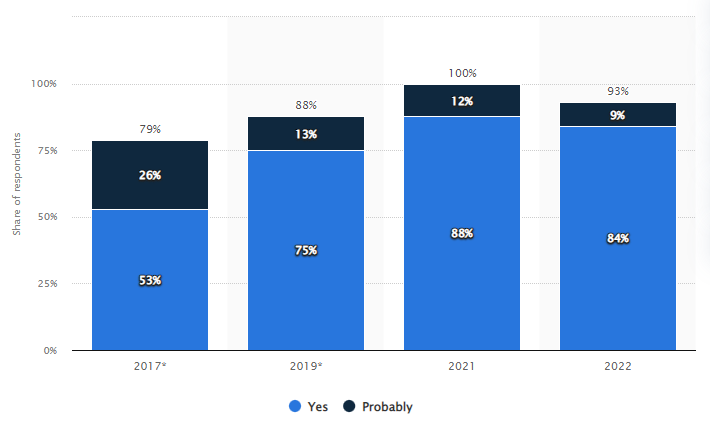
\includegraphics[width=1\textwidth]{gfx/Picture/Cyber_Crime.PNG}
 \caption{Eine Umfrage von deutschen Unternehmen, die von Daten Diebstahl, Espionage oder Sabotage betroffen waren. \cite{Stat22}}
 \label{fig:Crime}
\end{figure}

Wie man in der Grafik (\ref{fig:Crime}) erkennen kann, waren 88\% der befragten Unternehmen in Deutschland von Datendiebstahl, Espionage oder Sabotage in 2021 betroffen.
In 2022 lag die Zahl bei 84\%.
Wobei man berücksichtigen muss, dass diese Befragung zwischen Januar und März stattgefunden hat und dies daher nur das erste Quartal von 2022 abdeckt.
Aufgrund dessen, dass solche Angriffe wahrscheinlich sind, darf es keine "`Super Accounts"' geben, da diese ansonsten in solchen Angriffen als Schwachstelle ausgenutzt werden könnten.
Genauso müssen die Strukturen übersichtlich sein, damit bei einer Überprüfung es keine Probleme darstellt, festzustellen, welcher Nutzer welche Berechtigungen hat.
Wenn dies nicht der Fall ist, kann es passieren, dass die jeweiligen Nutzer zu viele Berechtigungen haben und dies wäre wieder ein Problem bei Espionage oder Sabotage.
Um dies zu erreichen, gibt es verschiedene Methoden und Konzepte, die die Berechtigungsstrukturen sicher und übersichtlich gestalten.

%
% Section: Ziele
%
\section{Ziel der Arbeit}
\label{sec:intro:goal}
Diese Arbeit ist eine Vergleichsarbeit, bei der verschiedene Konzepte verglichen werden.
Dabei wird auf die folgende Fragestellung in dieser Arbeit eingegangen, \textit{inwieweit kann man bestehende Berechtigungsstrukturen im Hostbereich verändern und optimieren kann}.
Dazu gibt es drei Unterfragen, welche verwendet werden, um die Problemstellung systematisch zu beantworten.

\begin{itemize}
  \item \textit{Welche Konzepte werden derzeit für Berechtigungsstrukturen verwendet, um diese sicher und übersichtlich zu gestalten?}
  \item \textit{Wie unterscheiden sich die verschiedenen Konzepte?}
  \item \textit{Womit kann man die verschiedenen Konzepte vergleichen?}
\end{itemize}

Die erste Unterfrage wird durch eine Recherche mit verschiedenen Arbeiten im Bereich der Berechtigungsstruktur beantwortet.
Dies soll einen Überblick zum Stand der Technik geben.
Anschließend wurden mehrere Befragungen durchgeführt, um die bestehenden Konzepten nach den Wünschen der Befragten anzupassen.
Darauf basierend werden die bestehenden Methoden geranked und verglichen.
Dies beantwortet die zweite Unterfrage mittels des erstellten Vergleiches.
\newline
Um die dritte Frage zu beantworten, wird ein Schema verwendet, welches als eine Hilfestellung zur Konzeptauswahl dienen wird.
Zum Schluss wird eine Alternative zum bestehenden System vorgestellt.
Dies ist die Arbeit in visueller Form.
\newpage
\begin{figure}[h!]
\hspace*{-3cm}
 \centering
 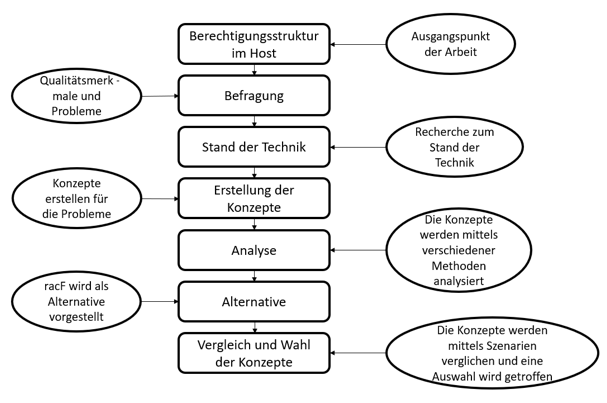
\includegraphics[width=1.5\textwidth]{gfx/Picture/Vorgehen.PNG}
 \caption{Aufbau der Arbeit}
 \label{fig:vorgehen}
\end{figure}
\newpage
\section{Ursache-Wirkungs-Diagramm}
\label{sec:intro:UWD}
\begin{figure}[h!]
 \centering
 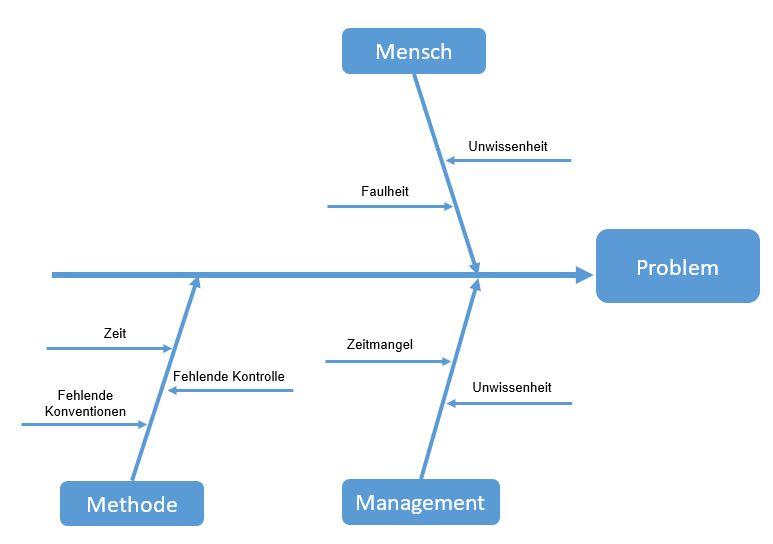
\includegraphics[width=1\textwidth]{gfx/Picture/Fisch.PNG}
 \caption{Ursache-Wirkungs-Diagramm (Fischgrätenmodell)}
 \label{fig:Fisch}
\end{figure}
Im Ursache-Wirkungs-Diagramm wurden dabei die folgenden drei Punkte als Hauptursache für das Problem der bestehenden Berechtigungsstruktur erkannt.
\begin{itemize}
	\item Mensch
	\item Management
	\item Methode
\end{itemize}
Bei Mensch sind die Mitarbeiter genannt, die die Berechtigungsstruktur verwalten und hegen.
Dort wurden die Punkte Faulheit und Unwissenheit genannt.
Dies liegt daran, dass es nicht unüblich ist, dass diese gewisse Formalien ignorieren, um einfacher das Problem zu beheben.
Auf der anderen Seite ist auch die Unwissenheit ein Problem, da die gesamte Struktur so gewachsten ist, ist es unmöglich für jemand diese komplett nachzuvollziehen.
\newline
Das Management hat nicht die Zeit, sich genau mit dem Problem zu beschäftigen.
Dies hat zur Folge, dass das Management wie die Mitarbeiter unwissend sind.
\newline
Bei der Methode steht die Zeit, fehlende Kontrolle und fehlende Konventionen als Problem dar.
Mit der Zeit ist gemeint, dass die aktuelle Problemstellung schon so lange der Fall ist, dass dies ein Problem ist.
An vielen Stellen fehlt bei der bestehenden Berechtigungsstruktur Kontrollen.
Dies ist zum Beispiel der Fall, wenn ein Account wieder aktiviert wird oder die Überprüfung von Profilen.
Denn wenn es diese gäbe, dürfte es keine rekursiven Beziehungen geben.
Es fehlt auch eine allgemeine Konvention, wie die Profile in den verschiedenen Fachbereichen funktionieren.
Dies sorgt dafür, dass es die Mitarbeiter schwerer haben alle Verbindungen zu verstehen und macht die gesamte Struktur komplexer.